\chapter{Empirical Study Design}
\label{Chapter3}
In this empirical study, our aim was to evaluate the effectiveness of the-state-of-art deep learning model (referred to as the Code readability enhancement model) proposed by Vitale \etal \cite{Vitale2023} in improving the readability of Java code. To accomplish this, we decided to extract and evaluate the readability of code samples before and after applying the model, utilizing a tool aimed at assessing and measuring the readability of a given piece of code. The objective was to understand if and how this model could enhance readability. Therefore, we extracted a set of Java code snippets and evaluated their readability both before and after applying the model. Our analysis focused on assessing any improvements in readability brought about by the model's interventions.\newline
Our study is steered by the following research questions:
\begin{itemize}
	\item \RQ{1}: What is the impact of applying automatic code readability enhancement considering snippets with varying levels of readability, namely low, medium and high?
\end{itemize}
With this inquiry, our aim is to understand how the model performs across various scenarios presented to it. The objective is to assess in which area the model excels most prominently and whether there are significant differences between the different scenarios.

\begin{itemize}
	\item \RQ{2}: Does readability enhancement through deep learning models change code behavior?
\end{itemize}
Here, we underscore the need to understand whether the model, by modifying the code, alters its behavior. This aspect is critical as it evaluates one of the essential aspects for proper refactoring practice, namely the preservation of code behavior.
\section{Experimental Procedure}
Our study is therefore based on an experimental approach aimed at answering two research questions, RQ1 and RQ2. To address these questions, we first need to obtain the data, which were collected from GitHub using its APIs. Once the data were obtained, we created the procedure to carry out the extraction phase of relevant parts (the methods of each class) and other information to generate the dataset that we will use as input for the model. This phase also serves as a foundation for the subsequent stages because it allows us to extract information about the position of the methods, the lines they are located on, and their class membership. Additionally, we use this phase to compute an initial assessment of the readability of the methods before they are modified by the model. To achieve this, we utilize the tool proposed by Scalabrino et al. \cite{Scalabrino2018}. During this phase, we also ensure to prepare and manipulate the methods to follow the input guidelines outlined by Vitale et al. \cite{Vitale2023}, and therefore, we apply a lexer to replace some characters with their respective tokens. Subsequently, we proceed with modifying the methods using the deep learning model offered by Vitale et al. We then move on to the manual evaluation and testing phase, where we manually filter the results (discarding obvious syntactic and/or semantic errors) and recalculate the readability score. By doing this, we can answer research question RQ1.\newline
To address RQ2, we will execute a patching phase, replacing the modified methods with the original ones, and then run the test suite of the projects under examination to understand if and how these changes have impacted the functionality of the procedure. This will allow us to determine if the behavior of the code has been altered.

As delineated above, our approach can be summarized as follows:
\begin{itemize}
	\item \textbf{Data collection}: we collected a dataset of Java projects from GitHub;
	\item  \textbf{Dataset creation}: we process the data in order to extract and tokenize the methods detected for our analysis and precompute the readability of those methods;
	\item \textbf{Model application}: we subjected the extracted methods to Vitale model in order to obtain the readability changes;
	\item \textbf{Manual evaluation and testing}: we manually evaluated the changes and tested the model's effectiveness in both readability and code alteration.
\end{itemize}

The pipeline of our approach is shown in Figure \ref{fig:pipeline}.
\begin{figure}[htbp]
	\centering
	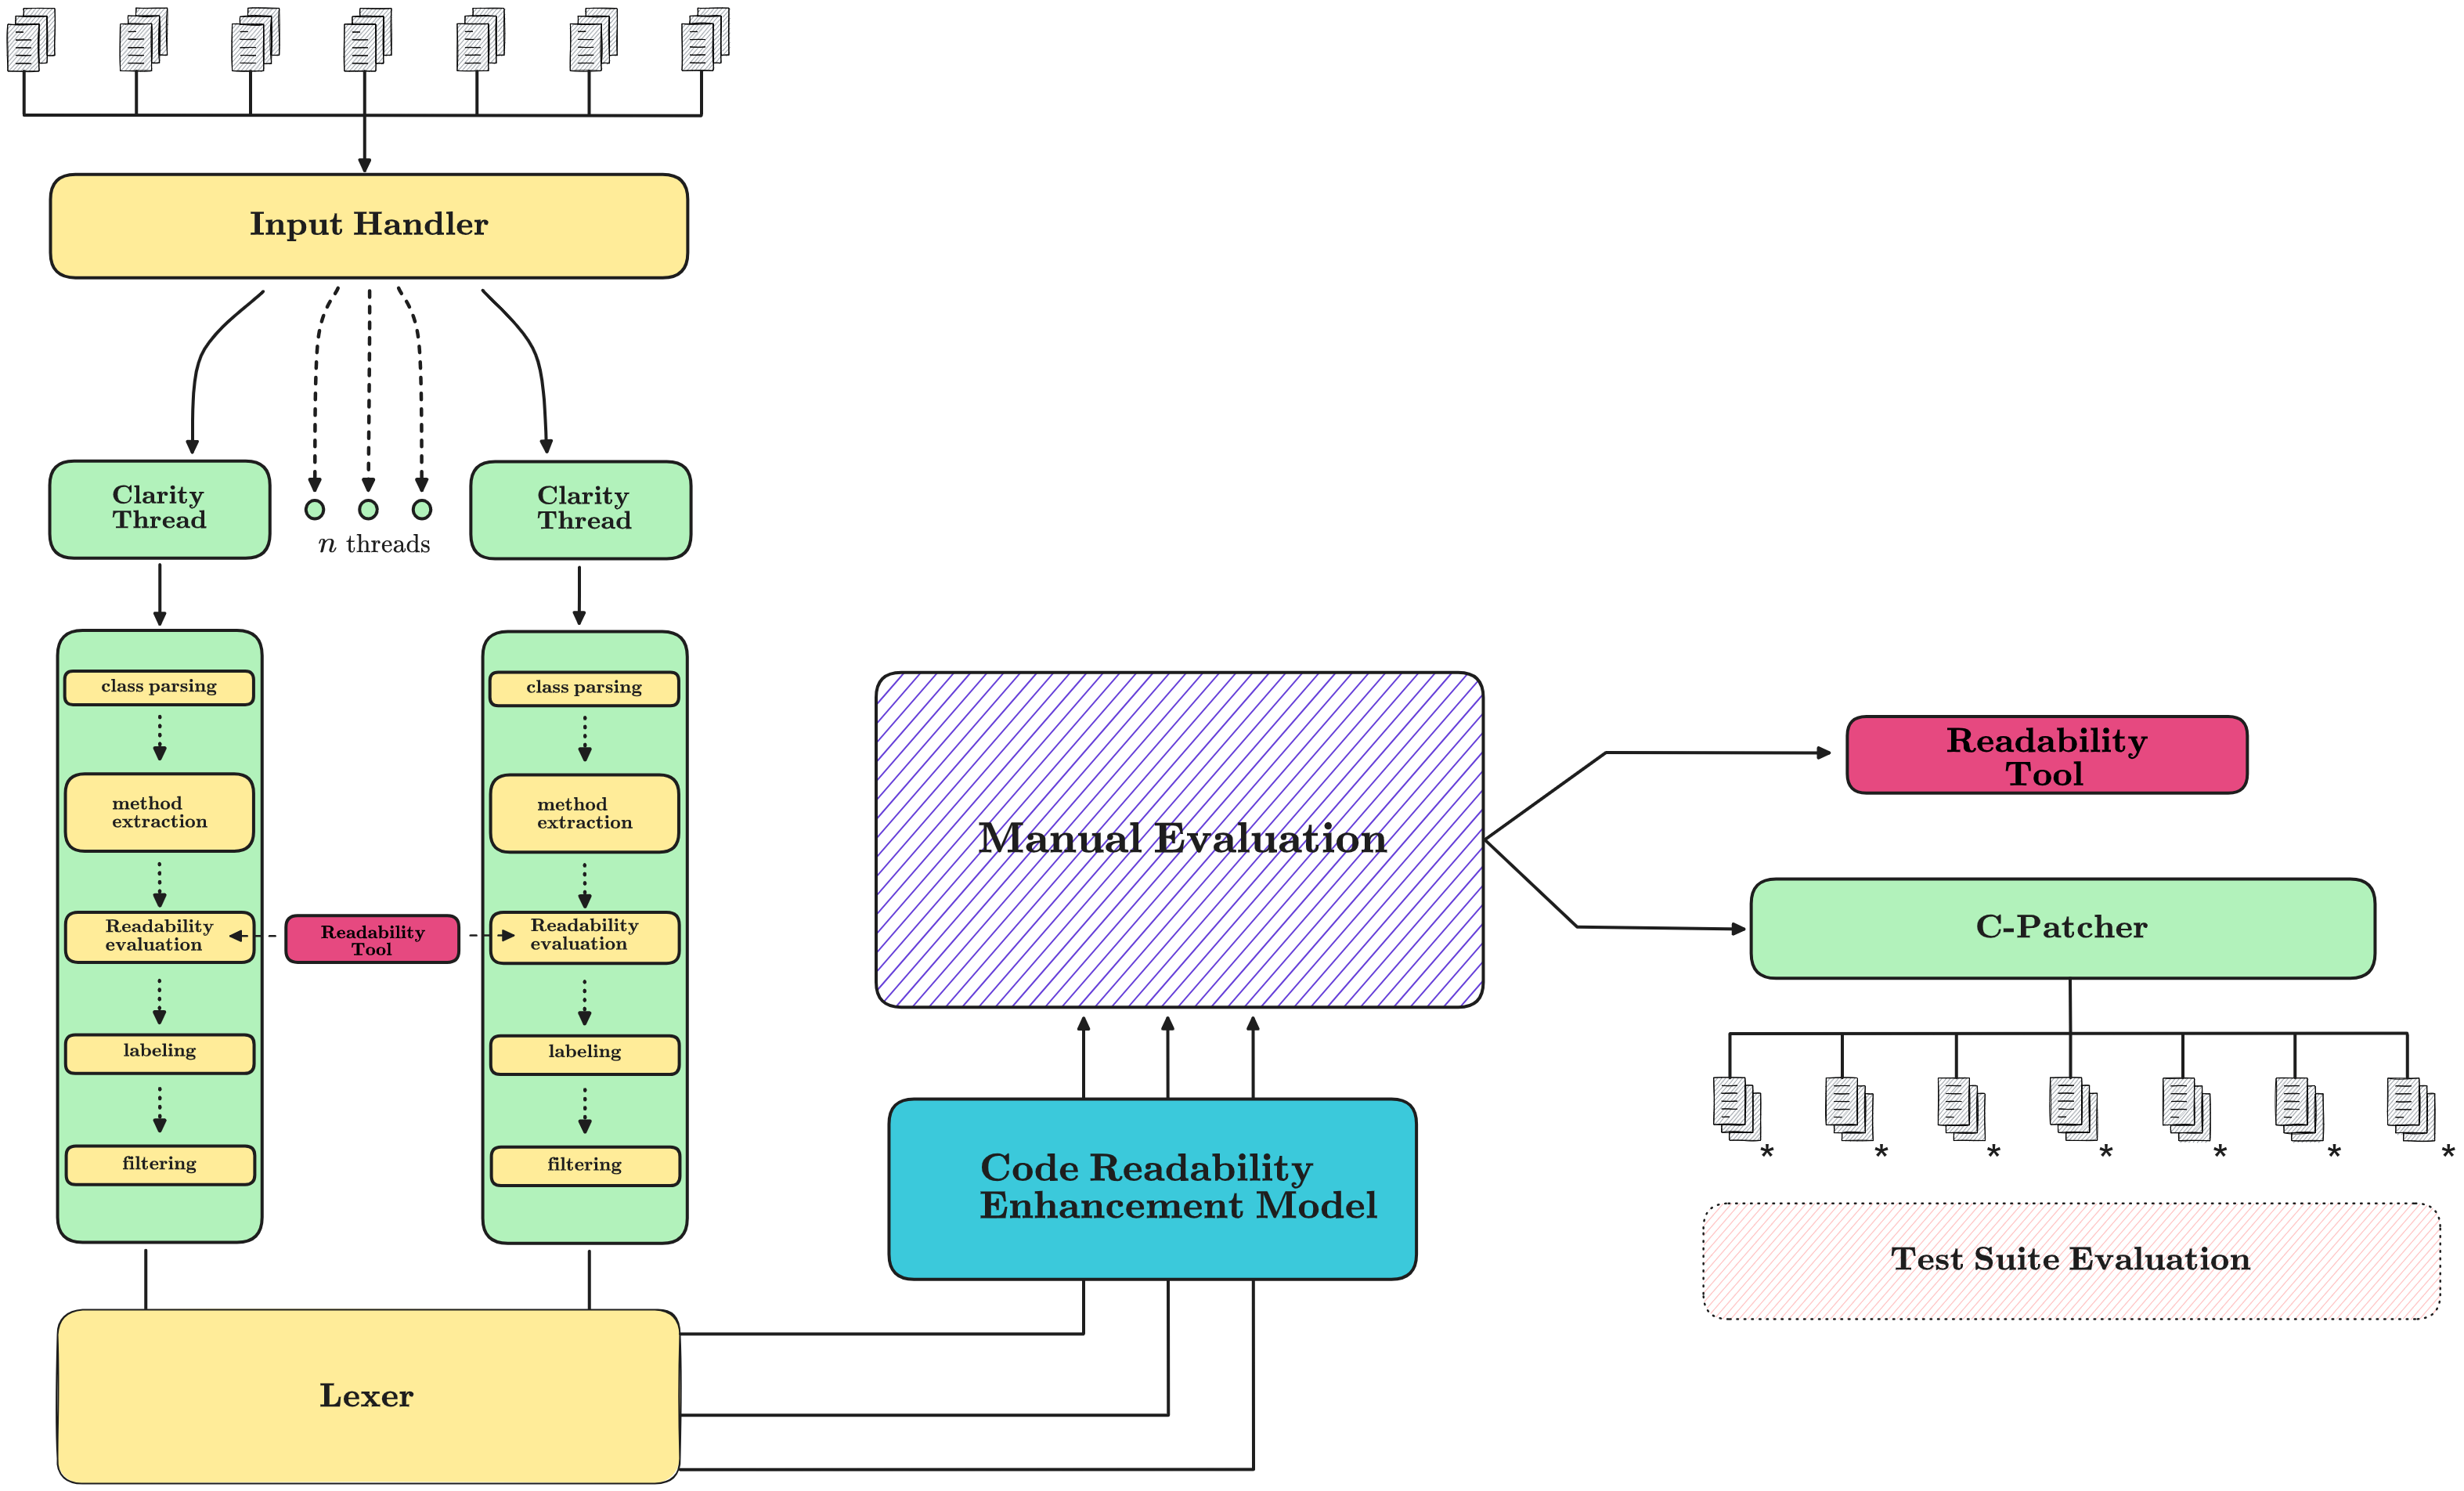
\includegraphics[width=1\textwidth,height=1\textheight,keepaspectratio]{figs/pipeline.png}
	\caption{}\label{fig:pipeline}
\end{figure}


\subsection{Data Collection}
In this phase, we utilized software repository mining techniques to extract the data essential for our research. We carefully selected three sizable Java projects, each actively maintained and equipped with a comprehensive test case suite. The chosen projects are:

\begin{itemize}
	\item \textbf{Guava}: an open source library from Google that provides a set of libraries useful for programming in Java;
	\item \textbf{Javaparser}: an open source library that allows you to analyze and manipulate Java source code;
	\item \textbf{Jenkins}: An open source automation system that provides support for building, testing, and deploying software.
\end{itemize}

\subsection{Data Preprocessing and Dataset Creation}
In this phase, our focus was on extracting methods from the selected projects. This approach was necessary because the insights gleaned from the Vitale et al. \cite{Vitale2023} study pertained specifically to Java code snippets, rendering reasoning at the class level impractical. To address this, we developed the "Clarity" tools, designed to extract methods from one or more Java projects, categorize them based on readability, and maintain a subset according to user-defined parameters. This tool comprises multiple components. Firstly, the Input Handler facilitates the analysis of multiple projects concurrently using multithreading techniques, primarily for optimization purposes. The Handler creates a set of threads corresponding to the number of input projects, with the user-defined numerical limit (defaulting to 4 threads) to prevent potential application crashes. Each thread executes a series of operations:

\begin{itemize}
	\item 1. \textit{Extract methods from java classes}
	\item 2. \textit{Evaluate methods readability }
	\item 3. \textit{Remove irrelevant results}
	\item 4. \textit{Labeling}
\end{itemize}
Which we will describe in detail in the next paragraphs.


\subsubsection{Methods Extraction} % (fold)
In this phase, we utilized the open-source tool \textit{Javaparser} to parse the Java classes, extracting the Abstract Syntax Tree (AST) a hierarchical representation of the structure of code that abstracts away details like spacing and formatting, which facilitated the identification of methods. From the extracted methods, we preserved crucial components including the declaration, body, annotations, and comments. Subsequently, as shown in Figure~\ref{code:dummy_class} this data was encapsulated within a dummy class and saved to file for further analysis.\newpage
\begin{lstlisting}[caption={Dummy Class}, label={code:dummy_class}, language = Java , frame = trBL , firstnumber = last , escapeinside={(*@}{@*)}]
public class DummyClass {
    //comments
    @Notation
    public void method() {
    }
}
\end{lstlisting}
To circumvent the extraction of "superfluous" methods, we implemented certain exclusions during this phase. Specifically, we chose to disregard getters and setters, as well as constructors. For the former two, we employed a heuristic based on the observation that getters and setters typically consist of no more than three lines. As for constructors, we leveraged the Javaparser API to identify and exclude them from the extraction process.
Although it is true that this heuristic may remove methods that are neither getters nor setters, we have still decided to use it. This decision is motivated by the fact that the likelihood of such methods containing readability errors is rather low, given the limited amount of code. Therefore, this explanation confirms the validity of the choice to exclude these methods.


\subsubsection{Readability Evaluation} % (fold)
\label{sub:Calculate readability}
To evaluate the readability of the Java methods, we utilized an API from a readability analysis tool developed as a result of the study conducted by Scalabrino et al. \cite{Scalabrino2018}. This tool offers an interface for analyzing the dummy classes generated during the extraction process. Through the analysis phase, by analyzing the code and taking into account different metrics such as line length, number of blank lines, periods etc. this tool produces a readability score \( s \) such that \( s \in [0,1] \), where:
\[
	\begin{aligned}
		0 & \implies \text{unreadable} \\
		1 & \implies \text{readable}
	\end{aligned}
\]
\newline
Once we obtained the score, we proceeded to save the necessary information for the tokenization and processing phase by the model. This data was saved in JSON format, retaining additional information required for later stages. Figure~\ref{code:method_info}is an example of the JSON structure:
\begin{lstlisting}[caption={Method's Information}, label={code:method_info}, language = json, frame = trBL , firstnumber = last , escapeinside={(*@}{@*)}]
{
  "name": "orNull",
  "method": "\t\t@Override\n\t\t@CheckForNull\n\t\tpublic T orNull(){\n\t\t    return null;\n\t\t}",
  "startLine": 64,
  "endLine": 68,
  "classPath": "guava/android/guava/src/com/google/common/base/Absent.java",
  "readabilityScore": 0.8923128247261047,
  "label": "NONE"
}
\end{lstlisting}
% subsection Calcolare la leggibilità (end)

\subsubsection{Data Filtering and Labeling} % (fold)
\label{sub:Labeling}
In the final phase of data extraction, considering the potentially vast number of methods generated by a large project, we opted to retain only a subset. Specifically, we selected the 20\% of the least readable methods, the 20\% of the average readable methods, and the 20\% of the most readable ones. To achieve this, we devised an algorithm that sorts the results based on the readability score and then filters out only the files meeting these percentage criteria. An example of the algorithm can be seen in Figure \ref{fig:filter_algorithm}.
As depicted, our decision was to retain not only the worst data, i.e., the least readable methods, but also the most readable and the averagely readable ones. This approach allows us to observe the model's performance across these three distinct scenarios.
\vspace{0.5cm}
\begin{figure}[H]
	\begin{center}
		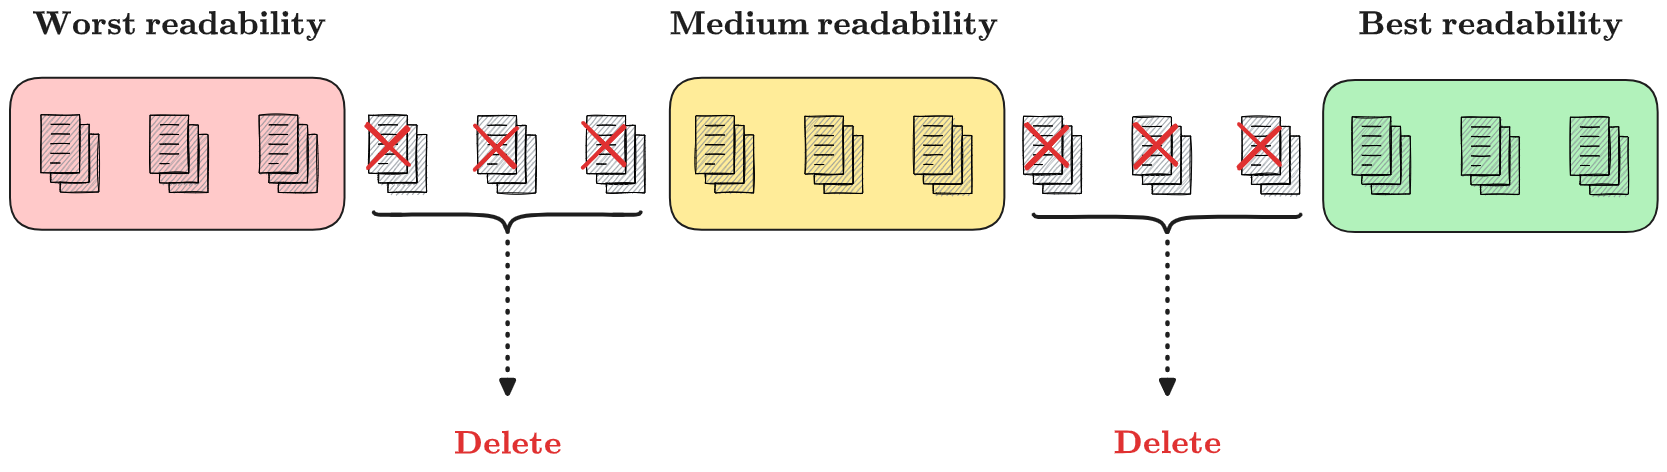
\includegraphics[width=0.95\textwidth]{figs/filter_algorithm.png}
	\end{center}
	\caption{}\label{fig:filter_algorithm}
\end{figure}


% subsection Labeling (end)
\subsubsection{Tokenization} % (fold)
\label{sub:Tokenization}
As mentioned, the model will take a series of methods as input and return an enhanced, more readable version. However, before proceeding with this, we need to pass our results through a lexer (lexical analyzer), which will enable us to divide the input text into meaningful sections known as tokens, representing the atomic units of the programming language. \newline
An example of tokenization is illustrated in the Table shown below:
\begin{table}[h!]
	\centering
	\begin{tabular}{|p{7cm}|p{7cm}|}
		\hline
		\textbf{Original Method}                      & \textbf{Tokenized Method}                                                                                                                                                                                                                                                                                                                                          \\
		\hline
		\begin{lstlisting}[language=Java, frame=none]
public void generate() {
    final int size = 0;
    final String alphabet = "";
    final String digits = "";
}
        \end{lstlisting} &
		\begin{lstlisting}[ frame=none]
public $whitespace$ void $whitespace$ generate ( ) $whitespace$ { $newline$ $indentation$ final $whitespace$ int $whitespace$ size $whitespace$ = $whitespace$ $number$ ; $newline$ $indentation$ final $whitespace$ string $whitespace$ alphabet $whitespace$ = $whitespace$ $string$ ; $newline$ $indentation$ final $whitespace$ string $whitespace$ digits $whitespace$ = $whitespace$ $string$ ; $whitespace$ 
        \end{lstlisting} \\
		\hline
	\end{tabular}
	\label{tab:tokenization}
	\caption{Comparison between the original method and the tokenized method.}
\end{table}
\newline
As evident, we eliminated extraneous characters such as spaces, newlines, and tabs, which convey text positioning but hold no significance for the language. Instead, we replaced them with specific tokens representing their behavior. Subsequently, we apply the theory described above to the set of JSON files obtained from the preceding steps to generate the input file for the model. The Ruby program responsible for the tokenization phase will generate, at the end, the Dataset in the form of a \textbf{\textit{TSV}} file.

\subsection{Model Application} % (fold)
In this phase, we processed the data obtained in previous phases using the deep learning model provided by Vitale et al. \cite{Vitale2023}. The model was accessible via a collaborative environment called \textit{Colab}, enabling the execution of Python instructions to configure the model and extract relevant data from the \textit{.tsv} file. Specifically, we focused on the \textit{tokenized\_method} field, containing the tokenized method, which served as input for the model. The model processed this data and returned a new tokenized method with readability changes, which we subsequently inserted back into the \textit{.tsv} file under a field named \textit{model\_prediction}\newline

\subsection{Data analysis} % (fold)
\label{sec:Data analysis}

From this point onward, we were almost equipped to address research questions \textit{RQ1} and \textit{RQ2}. We initiated an analysis of the data obtained to address these questions, starting with a manual evaluation of the model's responses to validate the results and ascertain if the model had indeed altered the instances. During this manual review phase, for the methods modified by the model, we manually replaced tokens that couldn't be automatically replaced, such as \textbf{\$string\$} and \textbf{\$number\$}. This manual replacement was necessary as the output of the model is not deterministic, thus making it impossible to automatically predict which string or number corresponds to which token. Additionally, during this manual phase, we also adjusted strings that were previously in uppercase, as the model, as currently defined, only provides predictions in lowercase.\newline
During this manual analysis, certain observations were made, and consequently, noticing a similar pattern in each modification, we decided to preserve a relatively small subset of the analyzed methods. Indeed, the total number (again 20\% of the total methods) amounted to approximately 5,000 methods per project. This number would have resulted in the need to manually analyze over 15,000 methods. To make the task more manageable, we decided to retain a sample of 100 methods per project. Additionally, to facilitate the modification of these methods, we decided to create a series of methodologies.
\begin{itemize}
	\item In series model result detokenization.
	\item Automatic camelCase conversion.
\end{itemize}
To address \RQ{1}, we needed to analyze the code provided by the model using Scalabrino \etal \cite{Scalabrino2018} tool. To accomplish this, we applied the detokenization phase, which was divided into two parts. The first part, automatic, dealt with replacing all tokens that could be replaced without manual intervention, such as \textbf{\$newline\$} or \textbf{\$indentation\$}. The second part was manual because we had to remove all tokens that could not be removed automatically. To facilitate this procedure, we introduced the first methodology which helped automate a component of this manual phase, namely the dataset manipulation. The second methodology was employed to expedite the process and reduce the manual effort required. By implementing this procedure, we decreased the potential for manual error introduction. This methodology, shown in Figure~\ref{fig:To camelCase algorithm}, involved converting the methods into CamelCase format. We developed a parser that generated a binary tree from the method under analysis. The algorithm precisely divides the input string into a list of strings using space as a delimiter and performs the following operations for each string:
\begin{itemize}
	\item 1. Set the string as the root of the tree.
	\item 2. Iterate through the string character by character, from left to right.
	\item 3. If we encounter a punctuation mark, set that mark as the root of the tree and the string preceding the mark as the left leaf. Then set the right node with the remaining unanalyzed string and recursively call the procedure on that node.
\end{itemize}
As we can observe, this algorithm defines an invariant that we can exploit to isolate words devoid of punctuation marks. Indeed, it will always be true that words lacking such marks will be found, for each subtree, either in a left leaf or at the root position. With this established, it was straightforward to reconstruct the original string by isolating the words that needed to be converted into CamelCase. For the conversion, we used a Python library called \textit{ninjaword}, which, employing a \textbf{N}atural \textbf{L}anguage \textbf{P}rocessing approach, successfully converted the strings into CamelCase with a reasonable success rate. It is worth noting that this library still has limitations. For example, the word "lightinglobe" can be correctly decomposed into multiple words, all equally valid: ["lighting", "globe"] or ["light", "in", "lobe"]. This highlights that, although this approach was simplifying in some respects, it certainly did not eliminate the need for manual analysis. Additionally, it's worth noting that this approach did not handle a certain type of keywords such as non-primitive data types since those types in Java start with an uppercase letter.
\begin{figure}[H]
	\begin{center}
		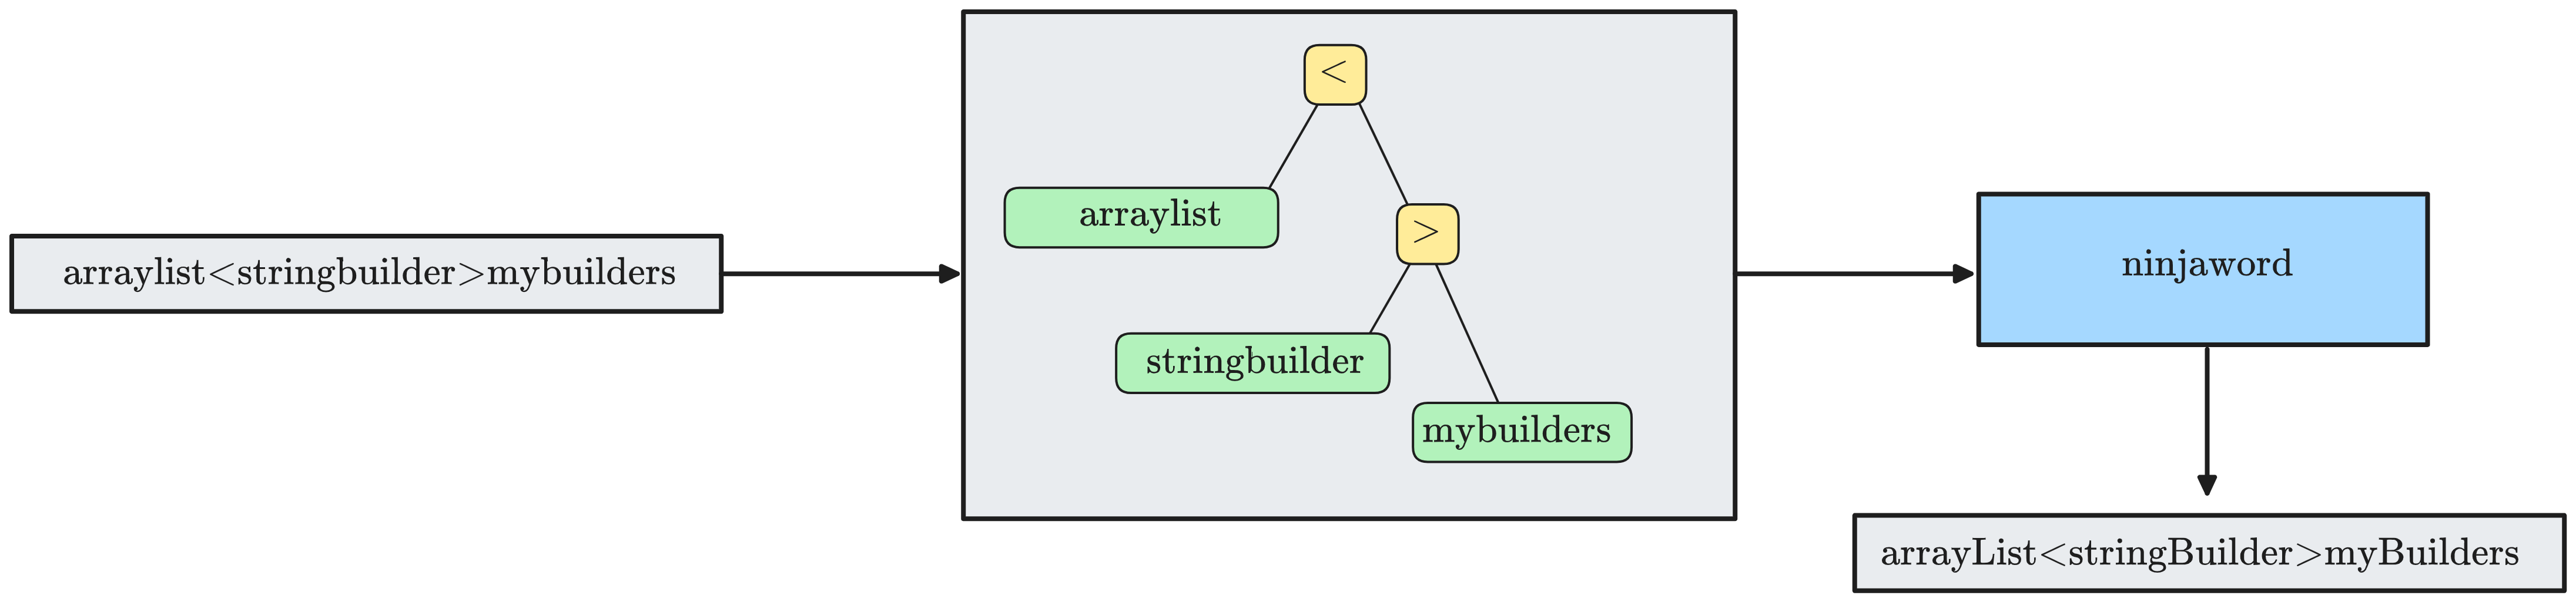
\includegraphics[width=0.95\textwidth]{figs/clay.png}
	\end{center}
	\caption{}\label{fig:To camelCase algorithm}
\end{figure}
The manual analysis removed a significant portion of the methods.
\begin{itemize}
	\item \textbf{Guava}: 67/100 methods were considered faulty
	\item \textbf{Jenkins}: 58/100 methods were considered faulty
	\item \textbf{Javaparser}: 58/100 methods were considered faulty
\end{itemize}
During this manual analysis, we corrected the syntax of certain methods by replacing tokens and rewriting procedures using the camelCase convention. Throughout this phase, we disregarded methods that were not modified by the model and discarded those deemed faulty. With "faulty," we mean that the method was not correctly modified by the model, thus resulting in syntax errors or even semantic errors, such as using an undeclared variable or omitting to return a value. \newline
During this analysis phase, we also manually indented the results. This was necessary because the model was trained in such a way that it could not distinguish 4-space indentations rather than 8-space indentations for the token \textbf{\$indentation\$}. However, this manual indentation did not significantly alter the model's output; rather, it ensured that each statement was properly aligned. This precaution was taken to prevent misinterpretations by the Scalabrino et al. tool \cite{Scalabrino2018}, and to ensure a more comfortable visualization.\\
We then executed Scalabrino \etal \cite{Scalabrino2018} tool to evaluate model prediction readability, and subsequently conduct a manual readability analysis, the objective was twofold: to identify minimal differences that the tool might have overlooked and to provide a secondary assessment of readability based on insights drawn from the work of Fakhoury et al. \cite{Fakhoury2019}. However, this secondary analysis does not rely on specific metrics but rather on perceived improvements as evaluated by the developer, namely myself. To address question \RQ{2}, we conducted a patching phase. Leveraging information about the class membership and the location of a given method within that class, obtained during the method extraction phase, it was straightforward to replace the original methods with the modified ones. Subsequently, we executed the test suite of the projects to understand if and how these changes impacted the functionality of the procedure. The execution of the test cases was atomic for each method, which means that, to prevent the modification of one method from impacting the results of another, we executed the test suite at every iteration of the patching procedure. This allowed us to determine whether the code behavior had been altered. The results of these analyses, along with other considerations, are reported in the next chapter.
% section Data analysis (end)

